\documentclass{article}
\usepackage[margin=1.35in]{geometry}
\usepackage{amsmath}
\usepackage{amsfonts}
\usepackage{amssymb}
\usepackage{amsthm}
\usepackage{parskip}
\usepackage{multicol}
\usepackage{xcolor}
\usepackage{fancyhdr}
\usepackage{physics}
\usepackage{graphicx} % Required for inserting images
\usepackage{hyperref}
\usepackage{biblatex}
\usepackage{tikz}
\usepackage{listings}
\usepackage{mwe}
\usepackage{caption}
\addbibresource{refer.bib}
\newcommand{\matr}[1]{\mathbf{#1}}

\title{
    $\text{Cu}_3\text{Au}$
    order-disorder entropy changes \\
    \large Thermodynamics Hand-in Project}
\author{Christopher Shen}
\date{November 2023}

\begin{document}

\maketitle

\tableofcontents
\newpage

\section{Introduction}

$\text{Cu}_3\text{Au}$ is an alloy that undergoes an order-disorder
(OD) transition from a $L1_2$ ordered face-centred cubic (fcc) with Cu
occupying the face centre to a disordered state in temperature range
$560K$ to $675K$\cite*{benisek}, as shown in figure 1.
This report aims to calculate the experimental and theoretical values of the
entropy change $\Delta S$ during this OD transition and attempt to
account for any discrepancies.
The entropy change of a material is important as other physical behavioural quantities
like the isobaric expansivity and $C_V$ may be predicted via the Maxwell's relations.

\subsection{Background theory}

\subsubsection{Entropy changes in OD transitions}
The total change in entropy from our OD transition is given by\cite*{paras}
$$\Delta S^{OD}=\Delta S^{vib}+\Delta S^{config}
+\Delta S^{mag}+\Delta S^{elec}$$
where $\Delta S^{vib}$ is the vibrational entropy change, 
$\Delta S^{mag}$ is the magnetic entropy change and
$\Delta S^{elec}$ is the electronic entropy change from disordering.
Finally $\Delta S^{config}$ corresponds to the theoretical entropy of mixing
and represents the entropy change when particles are rearranged 
from ordered fcc to a disordered state where there are still $4$ atoms per lattice
but their specific positions are now unknown.
Figure 1 below shows the ordered fcc structure of $\text{Cu}_3\text{Au}$
where $1/4$ of a Cu atom occupies the face centre
and $1/8$ of an Au atom occupies the vertices,
summing up to give $4$ atoms per lattice.

\begin{figure}[!htb]
    \centering
    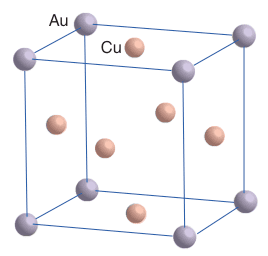
\includegraphics[scale=0.25]{f0.png}
    \caption{Ordered fcc $\text{Cu}_3\text{Au}$\cite*{inorg}}
\end{figure}

\subsubsection{Measuring $C_P$}
Here we outline the method for finding $\Delta S$
given data $C_P$ and temperature $T$. We define
$$C_P=\frac{\dd Q_p}{\dd T}=\left(\frac{\dd H}{\dd T}\right)_p$$
where state function $H$ is the enthalpy. Since $H=U+PV$:
$$\dd H=T\dd S+V\dd P$$
and dividing by $\dd T$:
$$\frac{\dd H}{\dd T}=T\frac{\dd S}{\dd T}+V\frac{\dd P}{\dd T}.$$
If $\Delta P=0$ then:
$$C_P(T)=T\left(\frac{\dd S}{\dd T}\right)_P.$$
Rearranging and integrating gives us the change in entropy:
$$\Delta S^{OD}=\int_{(1)}^{(2)}\frac{C_P(T)}{T}\dd T.$$

\newpage

\subsubsection{Ideal entropy of mixing}
Consider a box with separator, containing $n_A$ moles at $V_A$ of gas A on one side and $n_B$ moles at $V_B$ of gas B on the other. We set $\Delta T=0$, $\Delta P=0$ and proceed to \underline{mix} gases A and B.

The \textbf{entropy of mixing} is:
\begin{align*}
    \Delta S
    &=\Delta S_A+\Delta S_B \\
    &=n_i R\ln\left(\frac{V_f}{V_i}\right) \\
    &=n_A R\ln\left(\frac{V_A+V_B}{V_A}\right)
    +n_B R\ln\left(\frac{V_A+V_B}{V_B}\right).
\end{align*}
Since $P$ and $T$ are fixed, the ideal state equation $PV=nRT$ implies that:
$$\frac{V_A+V_B}{V_A}=\frac{n_A+n_B}{n_A}$$
and so we define \textbf{inverse mole fractions} as:
$$x_A=\frac{n_A}{n_A+n_B}$$
and
$$x_B=\frac{n_B}{n_A+n_B}.$$
After substituting and dividing through by $n_A+n_B$ we find the \textbf{molar specific entropy of mixing}:
$$\Delta s_{mix}=-R(x_A\ln x_A+x_B\ln x_B).$$
In the context of $\text{Cu}_3\text{Au}$ we have that:
\begin{align*}
    \Delta S_{mix}
    &=\Delta S^{config} \\
    &=-4R(x_{Cu}\ln x_{Cu}+x_{Au}\ln x_{Au}) \\
    &=18.7J\text{mol}^{-1}K
\end{align*}
where this is per $1$ mole of
$\text{Cu}_3\text{Au}$ and that $x_{Cu}=\frac{3}{4}$
and $x_{Au}=\frac{1}{4}$.

\newpage

\section{Data analysis}

\subsection{Visualisations}
The temperature $T$ and heat capacity $C_P$ data are from Benisek and Dachs.\cite*{benisek}
\\
Using the following Python code we can plot figures 2 and 3.
\begin{lstlisting}[language=Python]
    import pandas as pd
    import matplotlib.pyplot as plt

    df = pd.read_csv("data.csv")

    x = df["temp"]
    y1 = df["cp"]
    y2 = df["cp"] / x

    plt.plot(x, y1)
    plt.show()
\end{lstlisting}

\captionsetup[figure]{font=small,labelfont=small}
\begin{figure}[!htb]
    \centering
    \begin{minipage}{0.45\textwidth}
        \centering
        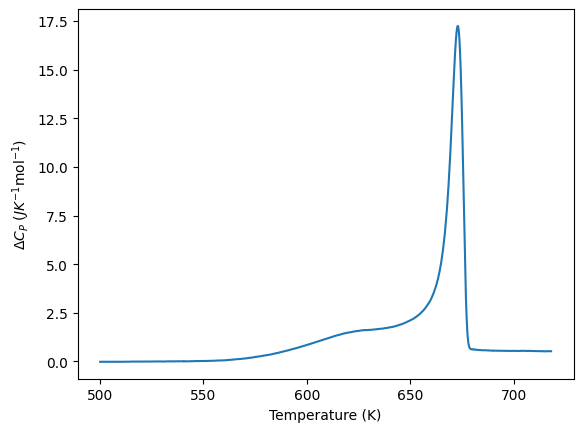
\includegraphics[scale=0.43]{f1_cp.png}
        \caption{$\Delta C_P$ ($JK^{-1}\text{mol}^{-1}$)
        against $T$ ($K$)}
    \end{minipage}\hfill
    \begin{minipage}{0.45\textwidth}
        \centering
        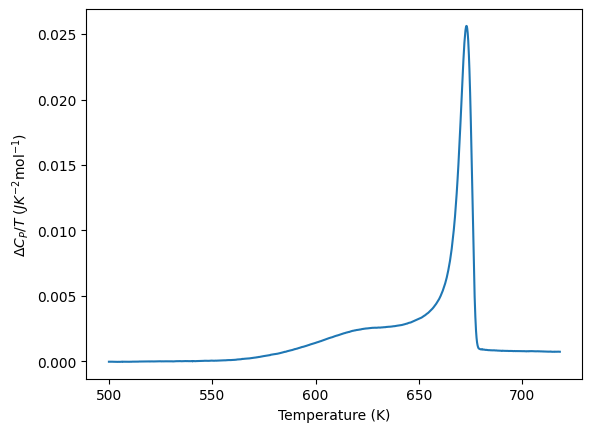
\includegraphics[scale=0.43]{f2_cp_over_t.png}
        \caption{$\displaystyle\frac{\Delta C_P}{T}$ ($JK^{-2}\text{mol}^{-1}$)
        against $T$ ($K$)}
    \end{minipage}
\end{figure}
It can be shown that there is a peak
near $T=680K$ using the following code:
\begin{lstlisting}[language=Python]
    import numpy as np

    i1 = np.argmax(y1)   # finds index of max value
    print(x[i1])

    i2 = np.argmax(y2)
    print(x[i2])
\end{lstlisting}
which gives the following outputs:
\begin{lstlisting}[language=bash]
    > 672.96
    > 672.96
\end{lstlisting}
The slight difference in temperatures ($673K$ compared to $680K$) are the result of
either experimental precision or that our peak occures
in a range of values rather than a specific temperature.

\newpage

\subsection{Calculating $\Delta S^{OD}$}
From before we have the following integral on endpoints $[a,b]$:
\begin{align*}
    \Delta S^{OD}
    &=\int_{a}^{b}\frac{C_P(T)}{T}\dd T \\
    &\approx\sum_i\frac{C_P(t_i)}{t_i}\delta t_i
\end{align*}
where given the $i$th datum of data 
we have that $\delta t_i=t_{i+1}-t_i$
for $t_i\in[a,b]$
and holds $\forall i\in\{1,\dots,n\}$.
Here $n$ corresponds to the number of data entries.
This sum may be found using the following code:
\begin{lstlisting}[language=Python]
    df_int = pd.concat([x,y2],axis = 1)
    df_cut = df_int[df_int.temp.between(560, 675)]
    df_cut.columns = ['temp','cpt']

    temp = df_cut["temp"].tolist()
    cpt = df_cut["cpt"].tolist()
    l = len(temp)

    total_area = 0
    for i in list(range(1, l)):
        base = temp[i]-temp[i-1]
        height = cpt[i]
        area = base*height
        total_area += area
    print(total_area) # in units R
\end{lstlisting}
which gives the following output:
\begin{lstlisting}[language=bash]
    > 0.38718425519279304
\end{lstlisting}
This choice of endpoints $[560K,675K]$ is suggested by
Benisek and Dachs:
\begin{align*}
    \Delta S^{OD}
    &=\int_{560}^{675}\frac{C_P(T)}{T}\dd T \\
    &\approx 0.39R \\
    &=3.24JK^{-1}\text{mol}^{-1}
\end{align*}
where $R=8.31JK^{-1}\text{mol}^{-1}$ is the molar gas constant.
Choosing another set of endpoints:
\begin{align*}
    \Delta S^{OD}
    &=\int_{550}^{700}\frac{C_P(T)}{T}\dd T \\
    &\approx3.58JK^{-1}\text{mol}^{-1}
\end{align*}
and so after taking averages of the two we claim:
$$\Delta S^{OD}=3.41JK^{-1}\text{mol}^{-1}.$$

\newpage

\subsection{Physical interpretations}
Summarising our results we have that:
$$\Delta S^{OD}=\Delta S^{vib}+\Delta S^{config}
+\Delta S^{mag}+\Delta S^{elec}$$
for
$$\Delta S^{config}=18.7J\text{mol}^{-1}K
\hspace{0.1in}\text{and}\hspace{0.1in}
\Delta S^{OD}=3.41JK^{-1}\text{mol}^{-1}.$$
This suggests that some of the other entropies (vibrational,
magnetic and electronic) are negative valued,
confirmed via Paras and Allanore.\cite{paras}
They also note that
$\text{Cu}_3\text{Au}$ undergoes multiple stages of transitions
before disordering. ($I\rightarrow II\rightarrow D$)
Furthermore we have that $\text{Cu}_3\text{Au}(I)$ is an
orderd fcc and $\text{Cu}_3\text{Au}(II)$ a
tetragonal structure consisting of $18$ $\text{Cu}_3\text{Au}(I)$
unit cells.\cite{okamoto}
The disordered fcc state ($D$) for temperatures greater
than $T=675K$ can be thought of as a solid
"solution" of Cu and Au atoms where entropy change is computed
via ideal entropy of mixing.

\section{Conclusions}
This report calculates the ideal entropy of mixing and
compares it to the numerically integrated entropy value
from experimental data. It is then concluded that
the discrepancies between these two values were due
to other entropy values.
We also remark that improved quenching techniques
and experiemental data with higher precision will result in
a better data analysis.

\printbibliography[title={References}]

\end{document}